\section{Тригонометричний ряд Фур'є}

\subsection{Визначення тригонометричного ряду Фур'є}

\begin{theorem}[інтеграл від періодичної функції]
    Нехай $f: \RR \to \CC$ --- $T$-періодична на $\RR$ і $f \in L([0, T])$. Тоді $\forall \{a, b\} \subset \RR$: $f \in L([a, b])$ і 
    \begin{equation}
        \int_a^{a + T} f(x) \diff x = \int_0^T f(x) \diff x.
    \end{equation}
\end{theorem}

\begin{figure}[H]
    \centering
    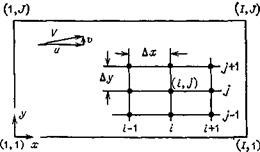
\includegraphics{01.png}
    \caption{Геометрична інтерпретація теореми: заштриховані площі рівні}
\end{figure}

\begin{proof}
    Спочатку доведемо, що $f$ інтегровна на $[a, b]$ для довільних $a$ і $b$. \medskip
    
    З періодичності $f$ маємо інтегровність $f$ на сегментах вигляду $[k T, (k + 1) T]$ для довільного цілого $k$:
    \begin{equation}
        \int_{k T}^{(k + 1) T} f(x) \diff x = \int_0^T f(x + k T) \diff x = \int_0^T f(x) \diff x.
    \end{equation}
    
    \begin{remark}
        Аналогічно можна отримати, що $f \in L([k T, m T])$ для довільних цілих $k < m$, причому 
        \begin{equation}
            \int_{k T}^{m T} f(x) \diff x = (m - k) \int_0^T f(x) \diff x.
        \end{equation}
    \end{remark}
    
    Далі, нехай $k$ --- таке, що $k T \le a < (k + 1) T$:
    \begin{figure}[H]
        \centering
        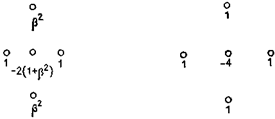
\includegraphics{02.png}
        \caption{Ілюстрація вибору $k$}
    \end{figure}
    
    Тоді, з адитивності інтегралу як функції множини, маємо:
    \begin{equation}
        \begin{aligned}
            \int_a^{a + T} f(x) \diff x
            &= \int_a^{(k + 1) T} f(x) \diff x + \int_{(k + 1) T}^{a + T} f(x) \diff x = \\
            &= \int_a^{(k + 1) T} f(x) \diff x + \int_{k T}^{a} f(x + T) \diff x = \\
            &= \int_a^{(k + 1) T} f(x) \diff x + \int_{k T}^{a} f(x) \diff x = \int_{k T}^{(k + 1) T} f(x) \diff x,
        \end{aligned}
    \end{equation}
    а цей інтеграл рівний бажаному.
\end{proof}

\begin{remark}
    Якщо $f(x)$ --- $T$-періодична, то $f(\frac{T x}{2 \pi})$ --- $2\pi$-періодична. Справді:
    \begin{equation}
        f \left( \frac{T (x + 2 \pi)}{2 \pi} \right) = f \left( \frac{T x}{2 \pi} + T \right) = f \left( \frac{T x}{2 \pi} \right).
    \end{equation}
\end{remark}

\begin{definition}
    $\{\frac{1}{2}, \cos x, \sin x, \cos 2x, \sin 2x, \ldots\}$ --- \textit{основна тригонометрична система}.
\end{definition}

\begin{definition}
    Довільна скінченна лінійна комбінація функцій основної тригонометричної системи --- \textit{тригонометричний многочлен}:
    \begin{equation}
        f(x) = \frac{a_0}{2} + \sum_{k = 1}^n (a_k \cos k x + b_k \sin k x).
    \end{equation}
\end{definition}

\begin{th_formula}[Ейлера]
    Виконуються наступні співвідношення:
    \begin{equation}
        \cos x = \frac{e^{ix} + e^{-ix}}{2}, \quad \sin x = \frac{e^{ix} - e^{-ix}}{2 i}.
    \end{equation}
\end{th_formula}

З використанням формули Ейлера можемо записати тригонометрчиний многочлен у вигляді
\begin{equation}
    f(x) = \frac{a_0}{2} + \sum_{k = 1}^n \left( a_k \frac{e^{ikx} + e^{-ikx}}{2} + b_k \frac{e^{ikx} - e^{-ikx}}{2 i} \right),
\end{equation}
або ж у вигляді
\begin{equation}
    \label{eq:1.1.9}
    f(x) = \sum_{k = -n}^n c_k e^{ikx},
\end{equation}
де
\begin{align}
    \label{eq:1.1.10}
    c_k &= \frac{a_k - i b_k}{2}, \\
    \label{eq:1.1.11}
    c_{-k} &= \frac{a_k + i b_k}{2},
\end{align}
а також $b_0 = 0$.

\subsection{Коефіцієнти тригонометричного многочлена}

\begin{theorem}[обчислення коефіцієнтів тригонометричного многочлена]
    Якщо $\forall x \in (-\pi, \pi)$ виконується \eqref{eq:1.1.9}, то коефіцієнти $c_k$ цього тригонометричного многочлена обчислюються наступним чином:
    \begin{equation}
        c_k = \frac{1}{2 \pi} \int_{-\pi}^{\pi} f(x) e^{-ikx} \diff x, \quad k = \overline{-n, n}.
    \end{equation}
\end{theorem}
\begin{proof}
    $\forall m = \overline{-n, n}$:
    \begin{equation}
        \begin{aligned}
            & \frac{1}{2 \pi} \int_{-\pi}^{\pi} f(x) e^{-imx} \diff x = \\
            &\quad = \frac{1}{2 \pi} \int_{-\pi}^{\pi} \sum_{k = -n}^n c_k e^{i(k-m)x} \diff x = \\
            &\quad = \frac{1}{2 \pi} \sum_{k = -n}^n c_k \int_{-\pi}^{\pi} e^{i(k-m)x} \diff x.
        \end{aligned}
    \end{equation}
    
    З інтегралів, що знаходяться у сумі лише один не рівний нулеві, а саме той, для якого $k = m$. При $k = m$ відповідний інтеграл дорівнює $2 \pi$, а тому
    \begin{equation}
        \frac{1}{2 \pi} \sum_{k = -n}^n c_k \int_{-\pi}^{\pi} e^{i(k-m)x} \diff x = \frac{1}{2 \pi} c_m (2 \pi) = c_m.
    \end{equation}
\end{proof}

\begin{corollary}
    Якщо $\forall x \in (-\pi, \pi)$ виконується \eqref{eq:1.1.9}, то коефіцієнти $a_k, b_k$ цього тригонометричного многочлена обчислюються наступним чином:
    \begin{align}
        \label{eq:1.1.15}
        a_k &= \frac{1}{\pi} \int_{-\pi}^{\pi} f(x) \cos kx \diff x, \\
        \label{eq:1.1.16}
        b_k &= \frac{1}{\pi} \int_{-\pi}^{\pi} f(x) \sin kx \diff x.
    \end{align}
\end{corollary}
\begin{proof}
    Справді, співвідношення \eqref{eq:1.1.10}, \eqref{eq:1.1.11} можна переписати у вигляді
    \begin{align}
        a_k &= c_k + c_{-k}, \\
        b_k &= \frac{c_{-k} - c_k}{i}.
    \end{align}
    
    Підставляючи у ці співвідношення результат теореми, отримуємо
    \begin{equation}
        \begin{aligned}
            a_k 
            &= \frac{1}{2 \pi} \int_{-\pi}^{\pi} f(x) e^{-ikx} \diff x + \frac{1}{2 \pi} \int_{-\pi}^{\pi} f(x) e^{ikx} \diff x = \\
            &= \frac{1}{2 \pi} \int_{-\pi}^{\pi} f(x) ( e^{-ikx} + e^{ikx}) \diff x = \\
            &= \frac{1}{\pi} \int_{-\pi}^{\pi} f(x) \left( \frac{e^{-ikx} + e^{ikx}}{2} \right) \diff x = \\
            &= \frac{1}{\pi} \int_{-\pi}^{\pi} f(x) \cos kx \diff x,
        \end{aligned}
    \end{equation}
    а також
    \begin{equation}
        \begin{aligned}
            b_k 
            &= \frac{1}{2 \pi i} \int_{-\pi}^{\pi} f(x) e^{ikx} \diff x - \frac{1}{2 \pi i} \int_{-\pi}^{\pi} f(x) e^{-ikx} \diff x = \\
            &= \frac{1}{2 \pi i} \int_{-\pi}^{\pi} f(x) ( e^{ikx} - e^{-ikx}) \diff x = \\
            &= \frac{1}{\pi} \int_{-\pi}^{\pi} f(x) \left( \frac{e^{ikx} - e^{-ikx}}{2 i} \right) \diff x = \\
            &= \frac{1}{\pi} \int_{-\pi}^{\pi} f(x) \sin kx \diff x.
        \end{aligned}
    \end{equation}
\end{proof}

\begin{definition}
    Функціональний ряд $\frac{a_0}{2} + \sum_{-\infty}^\infty (a_k \cos k x + b_k \sin k x)$ називається \textit{тригонометричним рядом}.
\end{definition}

\begin{definition}
    Якщо коефіцієнти тригонометричного ряду обчислені за формулами \eqref{eq:1.1.15}, \eqref{eq:1.1.16}, то ряд називається \textit{тригонометричним рядом Фур'є} функції $f(x)$, а його коефієінти --- \textit{коефіцієнтами Фур'є}.
\end{definition}

\begin{remark}
    У комплексій формі коефіцієнти Фур'є мають вигляд:
    \begin{equation}
        c_n = \frac{1}{2 \pi} \int_{-\pi}^\pi e^{-i n x} \diff x, \quad n \in \ZZ,
    \end{equation}
    а сам ряд ---
    \begin{equation}
        \sum_{-\infty}^\infty c_n e^{i n x}.
    \end{equation}
\end{remark}

\begin{exercise}
    Нехай $f(x) = \text{sgn}(x)$, $x \in (-\pi, \pi)$. Обчисліть її коефіцієнти Фур'є (декілька перших).
\end{exercise}

\subsection{Ряд Фур'є рівномірно неперервної функції}

\begin{theorem}[ряд Фур'є рівномірно неперервної функції]
    Якщо тригонометричний ряд збігається рівномірно на $\RR$ то він є рядом Фур'є своєї суми.
\end{theorem}
\begin{proof}
    Позначимо суму ряду $f$:
    \begin{equation}
        f(x) = \frac{a_0}{2} + \sum_{n = 1}^\infty (a_n \cos n x + b_n \sin n x), \quad x \in \RR.
    \end{equation}

    Також позначимо її складові $f_n$:
    \begin{equation}
        f_n(x) = a_n \cos n x + b_n \sin n x.
    \end{equation}

    Зрозуміло, що $\forall n \in \ZZ: f_n \in C(\RR)$. Тому $f \in C(\RR)$ як сума рівномірно збіжного ряду з неперервних функцій. \medskip

    Далі $f \in R([-\pi, \pi])$ як неперервна на компакті (тут $R([a,b])$ --- клас інтегровних за Ріманом на $[a,b]$ функцій). \medskip

    Знайдемо коефіцієнти Фур'є для функції $f(x)$. Для цього запишемо
    \begin{equation}
        \label{eq:1.1.25}
        f(x) \cos kx = \frac{a_0}{2} \cos k x + \sum_{n = 1}^\infty (a_n \cos n x + b_n \sin n x) \cos k x
    \end{equation}

    \begin{proposition}
        У припущенні рівномірної збіжності ряду можемо інтегрувати ряд почленно.
    \end{proposition}
    
    А наш ряд \eqref{eq:1.1.25} якраз рівномірно збіжний. Справді, розглянемо послідовність частинних сум $S_n(x)$. Умова рівномірної збіжності означає, що $\forall \epsilon > 0$: $\exists n_0$: $\forall n \ge n_0$ $x \in \RR$ $|f(x) - S_n(x)| < \epsilon$. Позначимо $\sigma_n(x) = S_n(x) \cos k x$. Тоді $|f(x) \cos k x - \sigma_n(x)| = |\cos k x| \cdot |f(x) - S_n(x)| \le |f(x) - S_n(x)| < \epsilon$. \medskip

    Повертаємося до пошуку коефіцієнтів Фур'є:
    \begin{equation}
        \begin{aligned}
            & \int_{-\pi}^\pi f(x) \cos k x \diff x = \\
            &\quad = \int_{-\pi}^\pi \frac{a_k}{2} \cos k x \diff x + \sum_{n = 1}^\infty \left( a_n \int_{-\pi}^\pi \cos n x \cos k x \diff x + b_n \int_{-\pi}^\pi \sin n x \cos k x \diff x \right) = \\
            &\quad = \frac{a_0}{2} \int_{-\pi}^\pi \cos k x \diff x + \sum_{n = 1}^\infty \left( \frac{a_n}{2} \int_{-\pi}^\pi ( \cos (n - k) x + \cos (n + k) x ) \diff x \right. + \\
            &\qquad + \left. \frac{b_n}{2} \int_{-\pi}^\pi ( \sin (n - k) x + \sin (n + k) x ) \diff x \right).
        \end{aligned}
    \end{equation}

    Зрозуміло, що всі доданки у сумах рівні нулеві, окрім $n = k$ у першій сумі, який якраз $\frac{a_n}{2} \cdot 2 \pi$. Враховуючи ще $\frac{1}{\pi}$  отримали якраз \eqref{eq:1.1.15}. Зрозуміло, що розглядаючи аналогічним чином $\frac{1}{\pi} \int_{-\pi}^\pi f(x) \sin k x \diff x$ отримаємо \eqref{eq:1.1.16}. А ще, при $k = 0$ маємо $\frac{a_0}{2}$.
\end{proof}
